\documentclass[12pt]{article}
\usepackage{hyperref}
\usepackage{graphicx}
\title{Monitoring Memory and CPU Usage for Processes in Linux}
\author{Jatczak, David \and McNabb, Trent}

\begin{document}
	
	\maketitle
	
	\section{Introduction}
	
	\subsection{Context}
	Addressing this issue requires knowledge of what information is relevant to the calculation of memory and CPU (Central Processing Unit) resources, and how to get that information. Specifically, knowledge of the Linux '/proc/' file is needed.
	
	\subsection{Problem Statement}
	Computer users who are used to Windows might use Ctrl+Alt+Delete when they wish to see which processes are running and how much of the system's resources those processes are consuming. They may not be comfortable using the terminal to run commands that would display that information, and they might prefer to see the information in a Graphical User Interface (GUI). We would like to write a program that we can make accessible via the Ctrl-Alt-Delete keyboard shortcut that resembles the Windows Task Manager. It should allow for a clear and easy view of which processes are running and what resources each process is using. It should be easy to terminate a running process.
	
	\subsection{Result}
	We have written a program that is called on our system using the Ctrl-Alt-Delete keyboard shortcut. The program uses a GUI to display the running processes and the percentage of CPU resources and memory used by each process. The program allows users to easily select and terminate processes.
	
	\subsection{Outline}
	The rest of this report is structured as follows: Section 2 presents background information, including information about calculating system resource usage by specific processes using the Linux '/proc/' file; Section 3 describes in detail the program that we have written, which is the result of this project; Section 4 evaluates the result of the project, primarily through a usability study; Section 5 is the conclusion.
	
	\section{Background Information}
	The Linux '/proc/' file system stores information about processes and also other system information. Each process has a directory in the '/proc/' file system\cite[p. 792]{text}. The directory is created at '/proc/[pid]/', where pid is the process identification number. Each of these directories include a 'stat' file, a 'statm' file, and a '/status' file. In addition to the information about each process, there is also system information, i.e. the '/proc/cpuinfo' file and the '/proc/meminfo' file.\\
	The Resident Set Size in the number of pages that the system currently has in real memory.
	If we multiply that by the page size, that gives the amount of RAM currently used by the process.
	If we divide that by the total amount of memory used by the system, that will give us the percentage of system memory used by the process.
	The calculation is:\\
	(Resident Set Size * Page Size)/(Total System Memory.)\\
	Information about the resident set size of a process can be found is '/proc/status/statm' \cite{manProc}.
	Information about the total system memory can be found in '/proc/meminfo' \cite{manProc}.\\

A CPU can either be running or idle.
If it is running, it can be running a user space program, or running the kernel \cite{scoutBlog}.
If you add the time it is running the kernel, plus the time it is running a user space program, plus the amount of time it is idle, you get what we will call the Total CPU availability.
The percentage of CPU usage by a process is the amount of time that the CPU is running that specific process, divided by the Total CPU availability multiplied by 100.
The percentage of total CPU usage is the amount of usage, divided the total CPU amount, multiplied by 100, where the amount of usage is the time running user space programs plus the time running kernel space programs.\\
The amount of time that a process has been running in user mode can be found in '/proc/pid/stat'. \cite{manProc}
The total time spent by the CPU running user space processeses and the amount of time running the kernel can be found in '/proc/stat' \cite{manProc}.\\
	
	
Shortcuts, also known as hotkeys, that give functionality to applications are typically handled by an event handler.
Whenever a user presses a key on an operating system, an event is made and sent out for the event handlers to handle.
There are many more types of events than key presses and key releases, such as mouse movements, and GUI events.
Event handlers are in event loops. Event loops are embedded in applications themselves and/or in the operating system. Simple processes such as shell tools do not typically have event handlers, but many modern applications do. The typical structure of an event loop is that goes through the queue of events it has, does what it needs and then chooses to dispatch the event or not, afterwards waiting for more events. 

The Qt framework offers a library that gives GUI functionality and is based in C++, but it also used in other languages such as Python where it has been ported.
The Qt framework has an event loop and receives its events from windowing systems such as X11 or Wayland.
If you are interested in this topic, it is explained further by Thiago Macieira in his powerpoint on the Qt event loop\cite{QtSlides}.

For this text, we use X11 as our window system.
X11 is the base of the GUI system for Linux.
It handles all the communication between the user input and other windows because it is the framework that other applications are working off.
X11 has its own event loop, and is basically at the top of the hierarchy of event loops.

To interact with X11's event loop, you require a library such as Xlib or XCB.
XLib was made by the same company that created X11.
XCB is a faster alternative to Xlib and is asynchronous.
Both of these libraries communicate with X11 via binary because X11 uses a client-server design for its system.


	
\section{Result}

The GUI layout was created in QT Designer, which outputs a '.ui' file, which is an file in XML (Extensible Markup Language).
That '.ui' file is compiled by PyQt5 into the files that run the GUI.
For our program, those files were 'mainwindow.cpp', 'mainwindow.h', and 'mainwindow.cpp', and the python class that allows our program, 'Overseer.py', to interface with the gui, 'UImainwindow.py'.
'Uimainwindow.py' has a class called Ui\_MainWindow that allows the creation of Ui\_MainWindow objects.
These files are all generated by the PyQt5 compiler, and any changes in them are made by changing and recompiling the '.ui' file.
When the main function is run in 'Overseer.py', it creates an Ui\_MainWindow object, runs the OverseerMainWindow function and tells the Ui\_MainWindow object to show on the screen.\\
The OverseerMainWindow function creates the the model for the table that holds the data so that the UI can display it.
It creates an instance of the Proc class from 'proc.py'.
The OverseerMainWindow function calls the udpate function, which updates the data by calling the readData function on the Proc object and then updates the view by calling the updateView function.
It repeats this once every second.\\
The Proc object stores the following data: a dictionary called processList, a UserList object called userList, from 'userlist.py', an integer called totalMem, and two lists called cpu and openWindows.\\
The readData function runs the functions that populate each of those data members.
readTotalMem gets the total memory usage from '/proc/meminfo/'.
See Figure ~\ref{figTotalMem}.
The circled data is the data stored as totalMem.
\begin{figure}[h]
	\centering
	\textbf{Total Memory}\par\medskip
	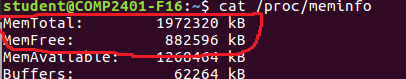
\includegraphics{totalMem}
	\caption{Output of 'cat /proc/meminfo'}
	\label{figTotalMem}
\end{figure}

readCupTimes gets the CPU infomation from '/proc/stat'.
See Figure ~\ref{figCPUInfo}.
The circled data are the numbers put in the list cpu.
The circled data are the numbers put in the list cpu.
This in the combined data for all processors in the system.
The first number is the time spent in user mode, and it is stored in cpu[0]
The third number is the time spent in system mode, and it is stored in cpu[3]
The fourth number is the time spent in idle, and it is stored in cpu[4].
None of the other numbers are relevant.
\begin{figure}[h]
	\centering
	\textbf{CPU Information}\par\medskip
	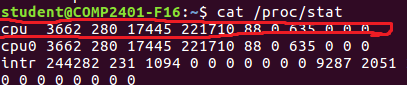
\includegraphics{totalCPU}
	\caption{Output of 'cat /proc/stat'}
	\label{figCPUInfo}
\end{figure}

IMPORTANT: I made this sound like a story and it must not sound like a story. Make sure to transform it.

Overseer is able to calculate its CPU usage and RAM usage through polling.
The interval for polling is every second.
Data is collected from all processes and the system.
This may seem like a strain, but there should not be overhead from IO blocking as files in /proc/ are virtual files and not actual files on a disk. Virtual files should be stored only on RAM (or replace as main memory or whatever).
With this, in theory you should be able to read all the info from /proc/ almost instantly.
Thus having 1 second of polling should not be too bad for the process.
When all this data is collected from /proc, we also perform our CPU and RAM usage calculations as well and also collect a list of users (at the start of the poll).
Collecting a list of users gives overhead as there is possible IO blocking from reading /etc/passwd as this is not a virtual file but a file on the disk.
Also obtaining window information through wmctrl might give overhead as well, and this data is collected in the poll cycle.

The original goal was to have Overseer launch upon startup and it would sit in the system tray, then it would show the window when the shortcuts ctrl+alt+del or ctrl+shift+esc was pressed.
There, it would have an event handler for checking for the shortcuts key press events of either Ctrl+Alt+Del and Ctrl+Shift+Esc.
If the key release event was detected for either shortcut before all 3 keys would get a keypress, the check for the shortcut would fail.
Implementation for putting a .desktop file in ~/.conf/autostart did manage to get the program to launch on startup, but if the user were to log out and log back in, it would not launch again.

However the main crux was the issue of reading events from X11 within the main Qt GUI thread.

Utilizing xlib to read key presses was doable.
The Qt framework only provided ways to add shortcuts if the Qt application itself was the focus (in focus).
The Qt framework is unable to read key presses when the Qt application is minimized or not in focus.
So another library was needed to read key presses, which led to Xlib.

However, due to lack of knowledge with xlib and the incredibly bad documentation with the python version of xlib.(the documentation was incredibly bad \url{http://python-xlib.sourceforge.net/doc/html/index.html}, also download the package python3-xlib and look in \url{/usr/share/doc/python3-xlib/html} and look how about the documentation is)

It was difficult to understand the example in \url{/usr/share/doc/python3-xlib/examples/}
\url{record_demo.py} as I had no idea how to reimplement the call back loop due to lack of documentation.

Essentially a call back loop would handle all the events in X11, then keep calling itself to handle more events.
It was not possible to implement this in the main Qt GUI thread because the GUI would stop working all together and look frozen.
It was thought it would be possible to implement the xlib call back loop as another thread, a QThread, so a 2nd thread would check for the shortcuts while the main Qt GUI thread would run.
However, xlib breaks (things and/or itself?) when used out of the main thread (I was told this by Thiago Macieira - Qt Core Maintainer on IRC).
Also multithreading is not a wise idea with Qt because it would just add more overhead to Qt's event loop (there's a web page talking all about this, it's hosted by Qt I think).

Thus XCB was turned to instead, as another way to read events.
A QAbstractNativeEventFilter was implemented to handle events straight from X11
The goal was to read \url{xcb_generic_event_t} that was passed by Qt into our handler.
However python does not recognize that type of data, and the PyQt5 library did not have an implementation of this data type either.
So an XCB library was needed to understand the \url{xcb_generic_event_t} data being sent by Qt's framework.
Due to our entire application being programmed in python 3.5.2, there were no decent libraries of XBC in python 3.5.2.
It was made for python 2.x
\url{https://xcb.freedesktop.org/XcbPythonBinding/}
A crawl over google led to other XBC implementations in pythyon 3.x such as /url{https://github.com/samurai-x/samurai-x/tree/master/pyxcb/pyxcb} or \url{https://github.com/tych0/xcffib}.
Both were failures in reading in \url{xcb_generic_event_t} for key presses even with some progress made into deciphering the event in \url{xcb_generic_event_t}.
But there were many missing functions and constant values such as \url{XBC_MOUSE_PRESS}.

Thus Ubuntu's custom shortcuts were used instead and we abandoned interacting with event handling. Overseer was made to no longer launch on startup, but instead a bash script was made instead where the Ubuntu shortcut would launch that, which in turn launched our Overseer application.
The custom shortcuts are separate for each each user and are located in ~/.config/dconf
The files are not plaintext, so the only way to change the configurations is through the terminal command 'gsettings'.
The implementation was successful and got the functionality we wanted.
However, the Ctrl+Shift+Esc shortcut does not work. The reason is in Ubuntu's shortcut manager not having Esc work as a shortcut at all\url{https://bugs.launchpad.net/ubuntu/+source/compiz/+bug/158855}.

For the applications tab, a 3rd party tool, wmctrl, was used to interact with windows in the window manager.
It collects the windows showing in desktop and also gives the functionality for switching to the windows.
Unfortunately it still collects junk windows like Unity's 'Hud', etc (check proc.py for the 'crap' comment for the list of them).

There is a fully functional right click menu and the buttons work. (Write whatever you want about this since there weren't failures with this)

Selections on the QtTableViews (process list \& applications list) had issues because python had no pointers.
So it was hard to use Model View Controller design for this because we could not link our data from the Proc class as a model to a QtTableView.
So when new data was grabbed, the whole QtTableView had to be erased and the selection had to reselected by iterating over the entire list in the table view and checking if the PID is the same as the selection before the update/poll.
This adds overhead to the process.

The Overseer application was programmed as single threaded, but Qt adds its own threads for whatever it needs to do.

(Remark on how the entire application wasn't able to be finished)



(\^ All the above can be seen from the branches global-shortcuts and global-shortcuts-method2)

	
	
	\section{Evaluation}
	Evaluation goes here.
	
	\section{Conclusion}
	
	\subsection{Summary}
	Summary and highlights.
	
	\subsection{Relevance}
	Relevance with respect to the course topic.
	
	\subsection{Future Work}
	Question for TA -- future work in the field of this project, or ways that the project application itself could be continued on.
	
	
	\setcounter{secnumdepth}{0}
	\section{Contributions of Team Members}
	
	\begin{thebibliography}{3}
	\bibitem{QtSlides} Thiago Macieira - Qt Core Maintainer \url{http://github.com/boostcon/cppnow_presentations_2013/blob/master/mon/qt_event_loop.pdf?raw=true}
	\bibitem{manProc} Proc(5) - Linux Manual Page
	\url{http://man7.org/linux/man-pages/man5/proc.5.html}
	\bibitem{text}{Tanenbaum, A. S. (2015). \emph{Modern operating systems.}}
	\bibitem{scoutBlog} Understanding Linux CPU stats \url{http://blog.scoutapp.com/articles/2015/02/24/understanding-linuxs-cpu-stats}
	\end{thebibliography}{}

\end{document}
